%%%%%%%%%%%%%%%%%%%%%%%%%%%%%%%%%%%%%%%%%%%%%%%%%%%%%%%%%%%%%%%%%%%%%%%%%%%%%%%%%
%
% Purpose:  Verification part of V&V for the Relative model
%
% 
%
%%%%%%%%%%%%%%%%%%%%%%%%%%%%%%%%%%%%%%%%%%%%%%%%%%%%%%%%%%%%%%%%%%%%%%%%%%%%%%%%

% \section{Verification}

%%% code imported from old template structure
\subsection{Inspection of Behavior in Integrated Testing}
\inspection{Inspection of LVLH and NED Verification Simulations}\label{inspect:Relative}
  The verification of the integrated behavior of the \RelativeDesc\ is performed by proxy in the verification of the \textref{\NEDDesc}{ch:NEDivv} and \textref{\LVLHDesc}{ch:LVLHivv}.  The performance of the simulations in these verification tests indicates that the \RelativeDesc\ is performing as expected at a crude, conceptual level (comparison against analytical results was not performed in this case). This result partially satisfies requirement~\ref{reqt:Relative}.  Requirement~\ref{reqt:Relative} is fully satisfied with the demonstration of performance against analytical results; this demonstration is provided in Test~\ref{test:Relative}. 


\subsection{Analytical Verification of Comprehensive Behavior in Unit Testing}

\test{Analytical Verification of \RelativeDescT\ Output Data for Multiple Scenarios}\label{test:Relative}

\begin{description}
\item[Purpose:]
To demonstrate that the data output by the \RelativeDesc\ provides accurate relative state information in simple, analytical  situations.

\item[Requirements:]
Satisfactory conclusion of this test partially satisfies requirement~\ref{reqt:Relative}.  Requirement~\ref{reqt:Relative} is fully satisfied with the additional demonstration of satisfactory performance within integrated testing; this demonstration is conducted at Inspection~\ref{inspect:Relative}.

\item[Procedure:]
A simulation was developed containing two vehicles in empty space.  Each vehicle
contained one vehicle-point.  Tests were run with the vehicles initialized in
various relative states, and the relative states between the points were
examined.  The state outputs were provided as the relative state of:
\begin{itemize}
 \item A with respect to B, expressed in reference frame B
 \item B with respect to A, expressed in reference frame A
\end{itemize}

\textbf{Notation:}
\begin{itemize}
\item 
Vectors are expressed numerically as a set of three values enclosed in square braces ($[x,y,z]$).
Subscripts on a vector denote the reference frame in which the values are expressed (i.e. which x,y,z axes are being used).
The subscripts used in this section are:
\begin{itemize}
 \item I - inertial
 \item SA - structural of vehicle A
 \item SB - structural of vehicle B
 \item PA - point frame of vehicle A
 \item PB - point frame of vehicle B 
\end{itemize}
\item Position, velocity and angular velocity are symbolically represented by:
\begin{itemize}
 \item $\vec x$ Position.
 \item $\vec v$ Translational velocity.
 \item $\vec \omega$ Rotational velocity.
\end{itemize}
\item Subscripts on the symbolic vector values are to be interpreted as follows ($P$, $Q$, and $R$ are used here as representatives of the frames used in this section):
\begin{itemize}
 \item $\vec x_{P}$ Position of frame $P$ (reference taken from context).
 \item $\vec x_{P|Q}$ Position of frame $P$ with respect to frame $Q$ (expression frame taken from context).
 \item $\vec x_{P|Q:R}$ Position of frame $P$ with respect to frame $Q$, expressed in frame $R$.
\end{itemize}
\item Conventionally,
\begin{itemize}
 \item $\vec x_{P|Q}$ is expressed in frame Q.
 \item $\vec v_{P|Q}$ is expressed in frame Q.
 \item $\vec \omega_{P|Q}$ is expressed in frame P.
\end{itemize}
\end{itemize}



The vehicles were configured as shown in Figure~\ref{fig:Relative_config}.  For
both vehicles, the respective structure and body frames are equivalent; the body frame will 
therefore not be mentioned again in this section.  

Vehicle B
is initially located such that $\vec x_{SB|I} = [0,0,0]_I$, with frame \textit{SB} aligned
with frame \textit{I}.  


Point B (the vehicle point on Vehicle B) is located at \newline
$\vec x_{PB|SB} = [1,0,0]_{SB}$ (initial conditions, $\vec x_{PB|I} = [1,0,0]_I$).
Frame \textit{PB} is initially rotated by -90 degrees
 about the z-axis with respect to frame \textit{SB}.

 Vehicle A is initially located such that $\vec x_{SA|I} = [10, 0, 0]_I$.  Its structural
 reference frame (\textit{SA}) is oriented with a +90 degree rotation about the z-axis from
 frame \textit{I}.  
 
 Frame \textit{PA}, associated with Point A,
 is located such that $\vec x_{PA|SA} = [1, 0, 0]_{SA}$ (initial conditions, $\vec x_{PA|I} =[10,1,0]_I$).
 It has a +90 degree rotation about the z-axis with respect to frame \textit{SA}.

 The dynamic states, where applicable, of the two vehicles are initialized such that:
 \begin{itemize}
   \item $\vec v_{SA|I} = [2 , 1 , 0 ]_I = [-2 , -1 , 0]_{PA}$
   \item $\vec \omega_{SA|I} = [0 , 9 , 0]_{SA}\ deg\ s^{-1} = [-9 ,
   0 , 0]_I\ deg\ s^{-1} = [9 , 0 , 0]_PA\ deg\ s^{-1}$
   \item $\vec v_{SB|I} = [0 , 0 , 1]_I$
   \item $\vec \omega_{SB|I} = [0 , 0 , 4.5]_I\ deg\ s^{-1}$ (same value in frames I,
   SB, PB).
 \end{itemize}

\begin{figure}[!ht]
 \begin{center}
  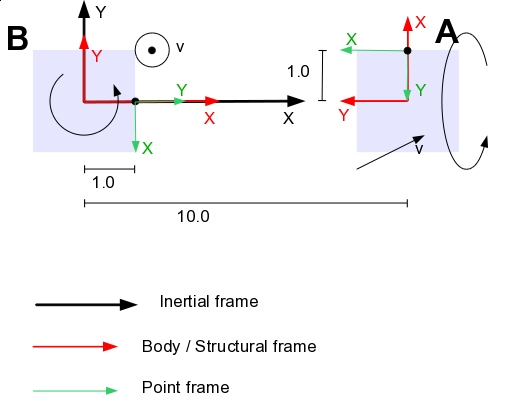
\includegraphics[width=80mm]{figures/relative_config.png}
  \caption{The configuration of the two vehicles and their respective reference frames.} 
  \label{fig:Relative_config}
 \end{center}
\end{figure}


Several simulation setups were considered, gradually increasing in complexity.

First, the rotational states were turned off, and only the effects of 
relative translational motion studied -- first one at a time, then both moving
together.
Then, the translational motion was zeroed, and only the effect of
relative rotational motion considered -- first one at a time, then both
together.
Finally, the situation in which both vehicles had translational and rotational
motion was considered.

\begin{enumerate}
 \item RUN\_no\_rot\_A\_trans
 \item RUN\_no\_rot\_B\_trans
 \item RUN\_no\_rot\_AB\_trans
 \item RUN\_A\_rot\_no\_trans 
 \item RUN\_B\_rot\_no\_trans
 \item RUN\_AB\_rot\_no\_trans  
 \item RUN\_AB\_rot\_AB\_trans  
\end{enumerate}

\item[Predictions:]



\begin{enumerate}
 \item RUN\_no\_rot\_A\_trans \newline
   With no rotation, the relative states are straightforward.  In this case, only vehicle A is moving.
   \begin{itemize}
    \item $\vec x_{PA|PB} = [(-1 - t), (9 + 2t) , 0]_{PB}$
    \item $\vec v_{PA|PB} = [-1 , 2 , 0]_{PB}$
    \item $\vec \omega_{PA|PB} = [0 , 0 , 0]_{PA}$
    \item $\vec x_{PB|PA} = [(9 + 2t) , (1 + t) , 0]_{PA}$
    \item $\vec v_{PB|PA} = [2 , 1 , 0]_{PA}$
    \item $\vec \omega_{PB|PA} = [0 , 0 , 0]_{PB}$
   \end{itemize}

 \item RUN\_no\_rot\_B\_trans \newline
 In this run, vehicle A is static, and vehicle B is moving.
 \begin{itemize}
    \item $\vec x_{PA|PB} = [-1 , 9 , -t]_{PB}$
    \item $\vec v_{PA|PB} = [0 , 0 , -1]_{PB}$
    \item $\vec \omega_{PA|PB} = [0 , 0 , 0]_{PA}$
    \item $\vec x_{PB|PA} = [9 , 1 , t]_{PA}$
    \item $\vec v_{PB|PA} = [0 , 0 , 1]_{PA}$
    \item $\vec \omega_{PB|PA} = [0 , 0 , 0]_{PB}$
   \end{itemize}
 \item RUN\_no\_rot\_AB\_trans \newline
 In this run, both vehicles have translational motion.
   \begin{itemize}
    \item $\vec x_{PA|PB} = [(-1 - t) , (9 + 2t) , -t]_{PB}$
    \item $\vec v_{PA|PB} = [-1 , 2 , -1]_{PB}$
    \item $\vec \omega_{PA|PB} = [0 , 0 , 0]_{PA}$
    \item $\vec x_{PB|PA} = [(9 + 2t) , (1 + t) , t]_{PA}$
    \item $\vec v_{PB|PA} = [2 , 1 , 1]_{PA}$
    \item $\vec \omega_{PB|PA} = [0 , 0 , 0]_{PB}$
   \end{itemize}
 \item RUN\_A\_rot\_no\_trans \newline
  In this run, vehicle A is rotating (bit has no translational motion).  Vehicle B is static.
  
  The motion of A with respect to B, expressed in B, is fairly
  straightforward.  On the y-axis, there is no motion.  On the x-axis, the
  motion starts at zero, and increases as A rotates around towards +x, and
  should follow a sine curve.  On
  the z-axis, the motion starts at a (negative) maximum, and slows, as in a
  negative cosine curve.
  
  In frame A, it is quite apparent that the x-value of the position of
  Point B (i.e. frame B) remains constant, at 9.0.  However, the motion of
  Point B on the y- and z- axes is less obvious.  Point B will clearly be moving
  relative to Point A in the inertial frame, but frame A is rotating at the
  same time.
  
  At any given time, the location of Point A with respect to the center of
  mass of vehicle A is $\vec x_{PA|SA} = [0, -1, 0]_{PA}$, since the y- and z-axes rotate with
  the vehicle.  Point B does not move relative to the vehicle center of
  mass, so must be at $\vec x_{PB|PA} = (9, 1, 0)_{PA}$ relative to frame A.  In other words,
  Point B DOES NOT MOVE in frame \textit{PA}.
       
  This can be illustrated by considering the relative position of \textit{PB} with respect to \textit{PA} in the inertial frame:
  \begin{equation*}
  \begin{split}
    \vec x_{PB|PA} &= [1\ ,\ 0\ ,\ 0]_I - [10\ ,\ \cos k_A t\ ,\ -\sin k_A t]_{I} \\
                 & = [-9\ ,\ -\cos k_A t\ ,\ \sin k_A t]_{I}
  \end{split}
  \end{equation*}

  where $k_A = \frac{2 \pi}{40}\ s^{-1} = 0.157\ s^{-1}$.
  
  With a rotation rate of 9 degrees per second, the rotation period is 40 seconds; there should be 2.5 rotations during the 100 second simulation).
   
     
  The transformation matrix from $I$ to $PA$ is a combination of a 180-degree z=rotation to begin, followed by a dynamic rotation on the x-axis:
  \begin{equation}
   \begin{split}
  T_{I\rightarrow PA} &=\begin{bmatrix} 1 & 0 & 0 \\ 0 & \cos k_A t & \sin k_A t \\  0 & -\sin k_A t & \cos k_A t \end{bmatrix}
  \begin{bmatrix} -1 & 0 & 0 \\ 0 & -1 & 0 \\ 0 & 0 & 1\end{bmatrix} \\
  &= 
  \begin{bmatrix} -1 & 0 & 0 \\ 0 & -\cos k_A t & \sin k_A t \\  0 & \sin k_A t & \cos k_A t \end{bmatrix}
  \end{split}
 \end{equation}\label{eqn:rel_verif_TIPA}

   Hence, applying the transformation matrix to the inertial expression yields:
   \begin{equation*}
   \begin{split}
        \vec x_{PB|PA} &= [9\ ,\ -\cos^2 k_A t -\sin^2 k_A t\ ,\ 0]_{PA} \\
                     &= [9\ ,\ 1\ ,\ 0]_{PA}
   \end{split}
   \end{equation*}

    \begin{itemize}
    \item $\vec x_{PA|PB} = [-\cos k_A t\ ,\ 9\ ,\ -\sin k_A t]_{PB}$
    \item $\vec v_{PA|PB} = [k_A \sin k_A t\ ,\ 0\ ,\ -k_A \cos k_A t]_{PB}$
    \item $\vec \omega_{PA|PB} = [9\ ,\ 0\ ,\ 0]_{PA}\ deg\ s^{-1}$
    \item $\vec x_{PB|PA} = [9\ ,\ 1\ ,\ 0]_{PA}$
    \item $\vec v_{PB|PA} = [0\ ,\ 0\ ,\ 0]_{PA}$
    \item $\vec \omega_{PB|PA} = [0\ ,\ 9\ ,\ 0]_{PB}\ deg\ s^{-1}$
   \end{itemize}

 \item RUN\_B\_rot\_no\_trans \newline
 In this scenario, vehicle B is rotating, and vehicle A is static.  The rotation axis of the rotating vehicle does not pass through the other vehicle's reference point, so the results are a little different to those from the previous test.
 
 The position and velocity of B with respect to A is easier, since the A frame is static.  For position, the x-value will oscillate between 9 and 11, starting at 9;  the y-value will oscillate between 0 and 2, starting at 1 and decreasing;  the z-value remains at 0 throughout.  For velocity:  the x-value starts at 0 and increases initially; the y-value starts at a minimum; z remains 0 throughout.  The angular velocity is a simple rotation on the z-axis.
 
 The position and velocity of A with respect to B is more challenging.  We start by considering the relative position in the inertial frame:
 \begin{equation*}
  \vec x_{PA|PB} = [10 - \cos k_B t\ ,\ 1 - \sin k_B t\ ,\ 0]_{I}
 \end{equation*}
 
 where $k_B = \frac{2 \pi}{80}\ s^{-1} = 0.0785\ s^{-1}$


 The transformation matrix from $I$ to $PB$ is a simple z-axis rotation matrix, since both the initial rotation and the dynamic rotation are on the z-axis:
  \begin{equation}
  T_{I\rightarrow PB} =\begin{bmatrix} \sin k_B t & -\cos k_B t & 0 \\ \cos k_B t & \sin k_B t & 0 \\ 0 & 0 & 1 \end{bmatrix}
 \end{equation}\label{eqn:rel_verif_TIPB}
 
 Hence,
 \begin{equation*}
  \vec x_{PA|PB} = [10 sin k_B t - cos k_B t , 10 cos k_B t + sin k_B t - 1 , 0]_{PB}
 \end{equation*}
 
 The velocity is the derivative of this expression.
 \begin{itemize}
    \item $\vec x_{PA|PB} = [10 \sin k_B t - \cos k_B t\ ,\ 10 \cos k_B t + \sin k_B t - 1\ ,\ 0]_{PB}$
    \item $\vec v_{PA|PB} = [10 k_B \cos k_B t + k_B \sin k_B t\ ,\ k_B \cos k_B t - 10 k_B \sin k_B t\ ,\ 0]_{PB}$
    \item $\vec \omega_{PA|PB} = [0\ ,\ 0\ ,\ -4.5]_{PA}\ deg\ s^{-1}$
    \item $\vec x_{PB|PA} = [10 - \cos k_B t\ ,\ 1 - \sin k_B t\ ,\ 0]_{PA}$
    \item $\vec v_{PB|PA} = [k_B \sin k_B t\ ,\ - k_B \cos k_B t\ ,\ 0]_{PA}$
    \item $\vec \omega_{PB|PA} = [0\ ,\ 0\ ,\ 4.5]_{PB}\ deg\ s^{-1}$
   \end{itemize}
   
   
 \item RUN\_AB\_rot\_no\_trans  \newline
 Combining the two rotations produces:
 \begin{equation*}
 \begin{split}
  \vec x_{PA|PB} &= [10\                   ,\ \cos k_A t\              ,\ -\sin k_A t]_{I} - 
                  [ \cos k_B t\         ,\  \sin k_B t\            ,\ 0]_{I} \\ 
               &=[10 - \cos k_B t\       ,\ \cos k_A t - \sin k_B t\ , -\sin k_A t]_{I}
 \end{split}
 \end{equation*}
 
 and, by symmetry,
 \begin{equation*}
  \vec x_{PB|PA} = - \vec x_{PA|PB}
 \end{equation*}
 
 Applying the transformation matrices (equations~\ref{eqn:rel_verif_TIPA} and~\ref{eqn:rel_verif_TIPB}) provides the relative positions in the appropriate frames.
  
  The translational velocity expressions are derived from the derivatives of the relative positions.
  The rotational velocity expressions are derived in a similar way to the translational positions.
  \begin{equation*}
  \begin{split}
  \vec \omega_{PA|PB} &= [-9\ ,\ 0\    ,\ 0]_{I} \ deg\ s^{-1}- 
                      [0\  ,\ 0\    ,\ 4.5]_{I}\ deg\ s^{-1} \\
                    &=[-9\ ,\ 0\    , -4.5]_{I}\ deg\ s^{-1}
  \end{split}
 \end{equation*}
  \begin{itemize}
    \item $\vec x_{PA|PB} = \begin{bmatrix} 10 \sin k_B t - \cos k_A t \cdot \cos k_B t \\
                                          10 \cos k_B t + \cos k_A t \cdot \sin k_B t - 1 \\ 
                                          -\sin k_A t
                          \end{bmatrix}
                          _{PB}$
 
    \item $\vec v_{PA|PB} = \begin{bmatrix} 
           10 k_B \cdot \cos k_B t + k_B \cdot \cos k_A t \cdot \sin k_B t + k_A \cdot \sin k_A t \cdot \cos k_B t\\
          -10 k_B \cdot \sin k_B t + k_B \cdot \cos k_A t \cdot \cos k_B t - k_A \cdot \sin k_A t \cdot \sin k_B t\\ 
            - k_A \cos k_A t
           \end{bmatrix}_{PB}$
    
    \item $\vec \omega_{PA|PB} = \begin{bmatrix} 9\\
                                               -4.5 sin k_A t\\
                                               -4.5 cos k_A t
                               \end{bmatrix}_{PA}\ deg\ s^{-1}$
    
    \item $\vec x_{PB|PA} = \begin{bmatrix} 10 - \cos k_B t\\
                                          1 - \cos k_A t \cdot \sin k_B t\\
                                          sin k_A t \cdot sin k_B t
                          \end{bmatrix}_{PA}$

    \item $\vec v_{PB|PA} = \begin{bmatrix} 
              k_B \sin k_B t \\
              k_A \cdot \sin k_A t \cdot \sin k_B t - k_B \cdot \cos k_A t \cdot \cos k_B t\\
              k_A \cdot \cos k_A t \cdot \sin k_B t + k_B \cdot \sin k_A t \cdot \cos k_B t\\ 
           \end{bmatrix}_{PA}$
           
    \item $\vec \omega_{PB|PA} = \begin{bmatrix} 9 \sin k_B t\\
                                               9 \cos k_B t\\
                                               4.5 
                               \end{bmatrix}_{PB}\ deg\ s^{-1}$
   \end{itemize}
  
 \item RUN\_AB\_rot\_AB\_trans  \newline
 With this run, the previously generated translational motion is added to the rotational motion; the same methods are applied (i.e. generate inertial expressions, transform to appropriate frame) to obtain the following expressions:
  \begin{itemize}
    \item $\vec x_{PA|PB} = \begin{bmatrix} 10 \sin k_B t - \cos k_A t \cdot \cos k_B t + t(2 \sin k_B t - \cos k_B t)\\
                                          10 \cos k_B t + \cos k_A t \cdot \sin k_B t - 1 + t(2 \cos k_B t + \sin k_B t \\ 
                                          -\sin k_A t - t
                          \end{bmatrix}
                          _{PB}$
 
    \item $\vec v_{PA|PB} = \begin{bmatrix} 
           \cos k_B t ( k_B (10+2t) + k_A (\sin k_A t) -1 )  + \sin k_B t (k_B(t + \cos k_A t) + 2) \\
           \cos k_B t (k_B(t + \cos k_A t) + 2) - \sin k_B t ( k_B (10+2t) + k_A (\sin k_A t) -1 )  \\ 
            - k_A \cos k_A t -1
           \end{bmatrix}_{PB}$
    
    \item $\vec \omega_{PA|PB} = \begin{bmatrix} 9\\
                                               -4.5 sin k_A t\\
                                               -4.5 cos k_A t
                               \end{bmatrix}_{PA}\ deg\ s^{-1}$
    
    \item $\vec x_{PB|PA} = \begin{bmatrix} 10 - \cos k_B t + 2t\\
                                          1 - \cos k_A t \cdot \sin k_B t + t (\cos k_A t + \sin k_A t)\\
                                          sin k_A t \cdot sin k_B t + t (\cos k_A t - \sin k_A t)
                          \end{bmatrix}_{PA}$

    \item $\vec v_{PB|PA} = \begin{bmatrix} 
              k_B \sin k_B t +2 \\
              \sin k_A t (k_A (\sin k_B t - t) +1) + \cos k_A t (1 + k_A t - k_B cos k_B t)\\
              \cos k_A t (k_A (\sin k_B t - t) +1) - \sin k_A t (1 + k_A t - k_B cos k_B t)\\ 
           \end{bmatrix}_{PA}$
           
    \item $\vec \omega_{PB|PA} = \begin{bmatrix} 9 \sin k_B t\\
                                               9 \cos k_B t\\
                                               4.5 
                               \end{bmatrix}_{PB}\ deg\ s^{-1}$
   \end{itemize}
\end{enumerate}

\item[Results:]
For test cases 1-4, the analytical solution is so simple that a simple inspection demonstrated that the results matched the predictions.  Test cases 5-7 required a little more analysis.  The results for test cases 6 and 7 are included below.  The results for test 5 were very similar.
 
 \begin{itemize}
  \item Test Case 6 \newline
  Figures~\ref{fig:rel6_1}-\ref{fig:rel6_4} show the differences between the analytical results and the numerical results for the two relative positions and the relative velocities.
   
   The results show very close agreement between the two sets of data.

 \item Test Case 7 \newline
  Figures~\ref{fig:rel7_1}-\ref{fig:rel7_6} show the differences between the analytical results and the numerical results for the two relative positions, velocities, and angular velocities.
   
   The results show very close agreement between the two sets of data.
  \end{itemize}
  
\item[Conclusion:]
In all cases, the numerical values very closely approximated the analytical values.  This test has demonstrated that the \RelativeDesc\ is correctly calculating the relative states when used in isolation.

In order to demonstrate that the model works identically regardless of whether or not it is associated with a Dynamic Body, an additional relative state was added to each of the test cases described above. It was identical in every way, in every scenario, to one of the already existing relative states, with the exception that it was initialized independently of any Dynamic Body. The generalized results proved to be a bitwise match to those for the pre-existing analog, and thus the results are not separately presented here.
  
 \begin{figure}[!ht]
  \begin{center}
        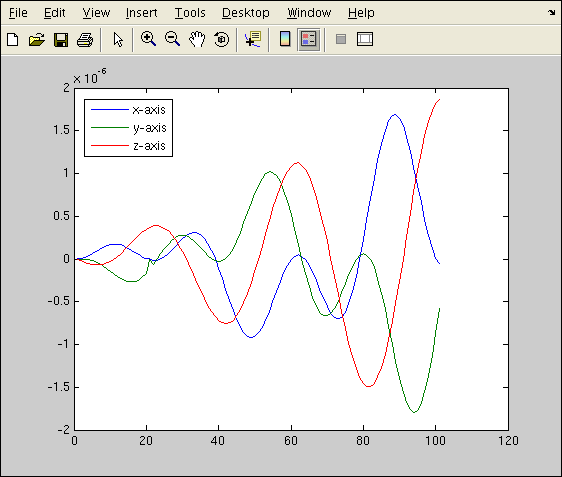
\includegraphics[width=80mm]{figures/relative6_xab.png}
        \caption{The variation with time of the difference between the analytical and numerical solutions for the position of A with respect to B.}
        \label{fig:rel6_1}
  \end{center}
\end{figure}

 \begin{figure}[!ht]
  \begin{center}
        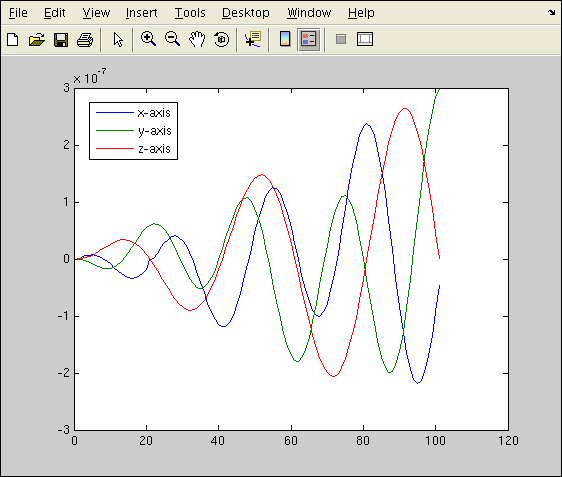
\includegraphics[width=80mm]{figures/relative6_vab.png}
        \caption{The variation with time of the difference between the analytical and numerical solutions for the velocity of A with respect to B.} 
  \end{center}
\end{figure}

 \begin{figure}[!ht]
  \begin{center}
        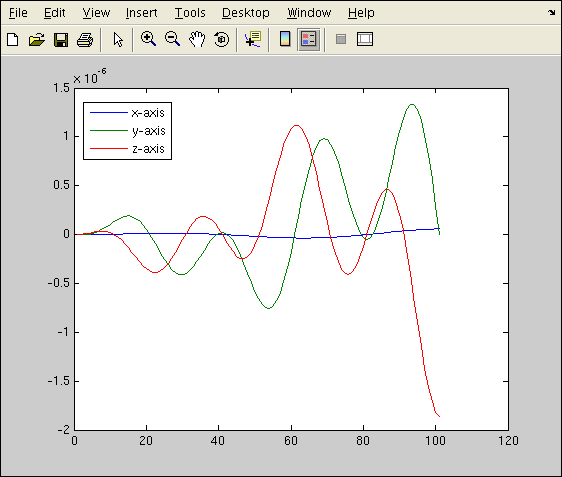
\includegraphics[width=80mm]{figures/relative6_xba.png}
        \caption{The variation with time of the difference between the analytical and numerical solutions for the position of B with respect to A.} 
  \end{center}
\end{figure}

 \begin{figure}[!ht]
  \begin{center}
        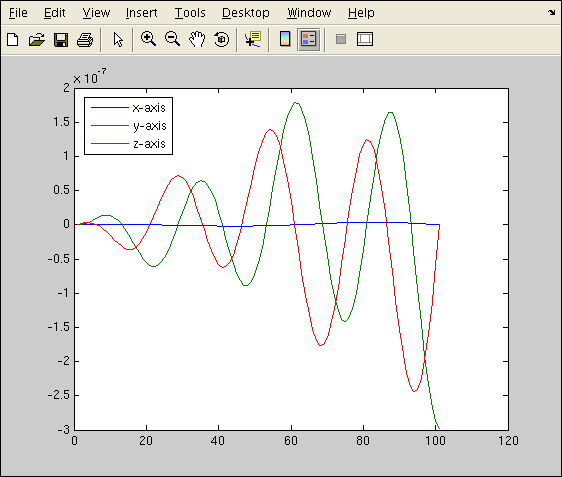
\includegraphics[width=80mm]{figures/relative6_vba.png}
        \caption{The variation with time of the difference between the analytical and numerical solutions for the velocity of B with respect to A.}
        \label{fig:rel6_4} 
  \end{center}
\end{figure}

 \begin{figure}[!ht]
  \begin{center}
        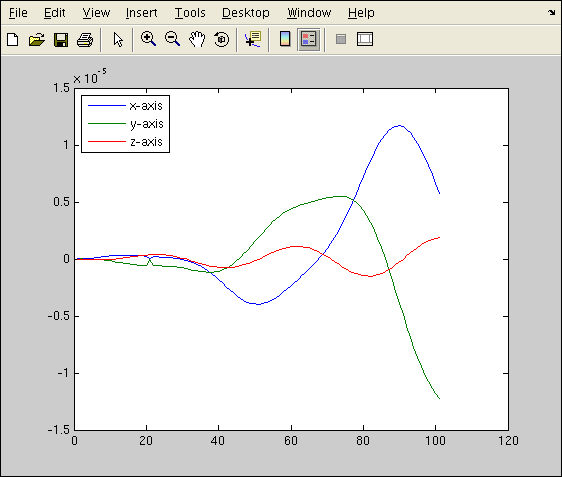
\includegraphics[width=80mm]{figures/relative7_xab.png}
        \caption{The variation with time of the difference between the analytical and numerical solutions for the position of A with respect to B.}
        \label{fig:rel7_1}
  \end{center}
\end{figure}

 \begin{figure}[!ht]
  \begin{center}
        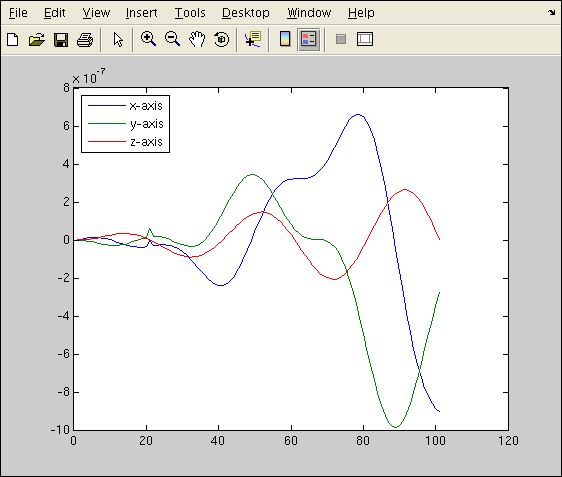
\includegraphics[width=80mm]{figures/relative7_vab.png}
        \caption{The variation with time of the difference between the analytical and numerical solutions for the velocity of A with respect to B.} 
  \end{center}
\end{figure}

 \begin{figure}[!ht]
  \begin{center}
        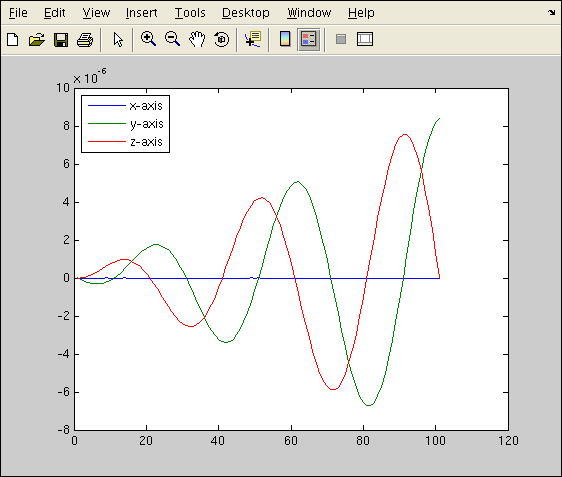
\includegraphics[width=80mm]{figures/relative7_wab.png}
        \caption{The variation with time of the difference between the analytical and numerical solutions for the angular velocity of A with respect to B.} 
  \end{center}
\end{figure}

\begin{figure}[!ht]
  \begin{center}
        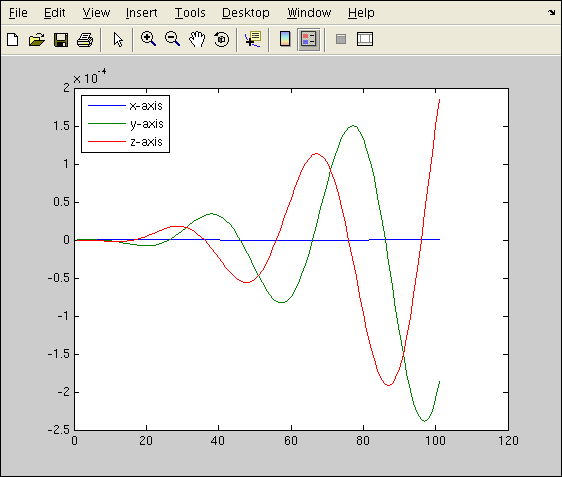
\includegraphics[width=80mm]{figures/relative7_xba.png}
        \caption{The variation with time of the difference between the analytical and numerical solutions for the position of B with respect to A.} 
  \end{center}
\end{figure}

 \begin{figure}[!ht]
  \begin{center}
        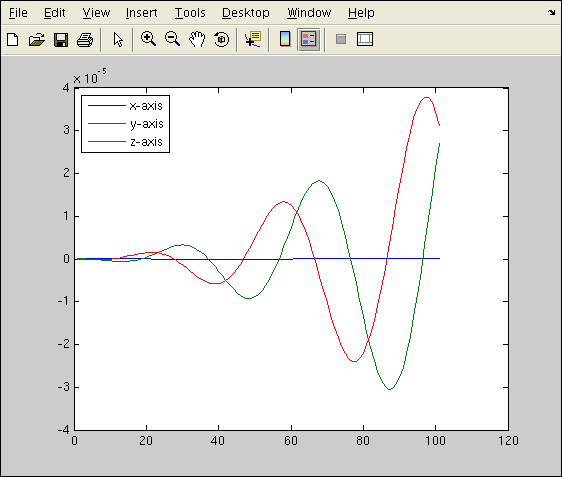
\includegraphics[width=80mm]{figures/relative7_vba.png}
        \caption{The variation with time of the difference between the analytical and numerical solutions for the velocity of B with respect to A.} 
  \end{center}
\end{figure}

\begin{figure}[!ht]
  \begin{center}
        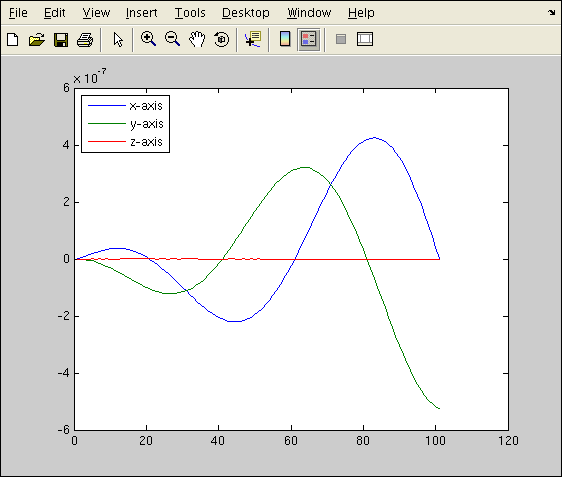
\includegraphics[width=80mm]{figures/relative7_wba.png}
        \caption{The variation with time of the difference between the analytical and numerical solutions for the angular velocity of B with respect to A.}
        \label{fig:rel7_6} 
  \end{center}
\end{figure}

\end{description}
